\documentclass{beamer}

\usepackage{beamerthemeblackboard}
\usepackage{graphics}
%\usepackage[pdftex]{graphicx}

\begin{document}

% set handwritten font, necessary packages are loaded in beamerthemeblackboard.sty
\ECFAugie

\begin{frame}
\title{Mariokart \\ An autonomous go-kart}
\author{Henry Jenkins}
\date{September 26, 2011}
\institute[2011]{Department of Computer and Electrical Engineering,\\
    University of Canterbury, \\ Christchurch, \\ New Zealand}
\maketitle
\end{frame}

\begin{frame}
\frametitle{Overview}
The Original Goal
\begin{itemize}
%\item ``The aim of this project is to take the departments go-karts and build in a
%system to replace the human driver. This will entail (at least), selection of
%appropriate actuators, motion and distance sensors, development of a navigation
%system, an interface to the existing control system, and a central computing
%platform. A suitable navigational goal would include a circumnavigation of S
%block.''
\item Make department go-kart drive autonomous
\item Have go-kart drive around uni
\end{itemize}

Our Goal
\begin{itemize}
\item Sub-goal of of drive-by-wire go-kart
\item Make a robust platform for future projects
\end{itemize}
\end{frame}

\begin{frame}
\frametitle{Project time line}
\framesubtitle{Gantt Chart}
    \begin{center}
      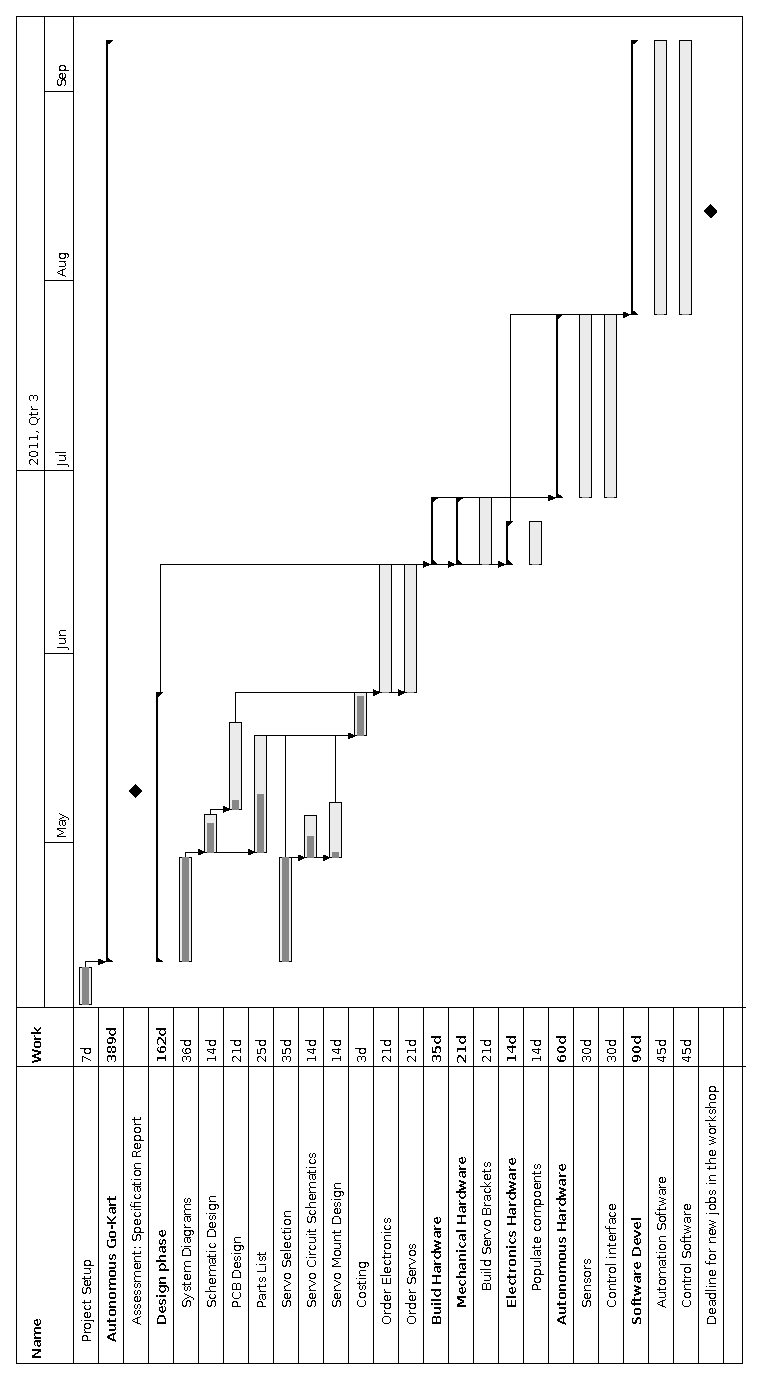
\includegraphics[angle=270,width=.95\textwidth]{Images/Gantt}
    \end{center}
\end{frame}

\begin{frame}
\frametitle{Hardware Layout}
\framesubtitle{Each board}
    \begin{center}
      \includegraphics[width=.95\textwidth]{Images/Hardware_block}
    \end{center}
\end{frame}

\begin{frame}
\frametitle{Hardware Layout}
\framesubtitle{Whole kart}
    \begin{center}
      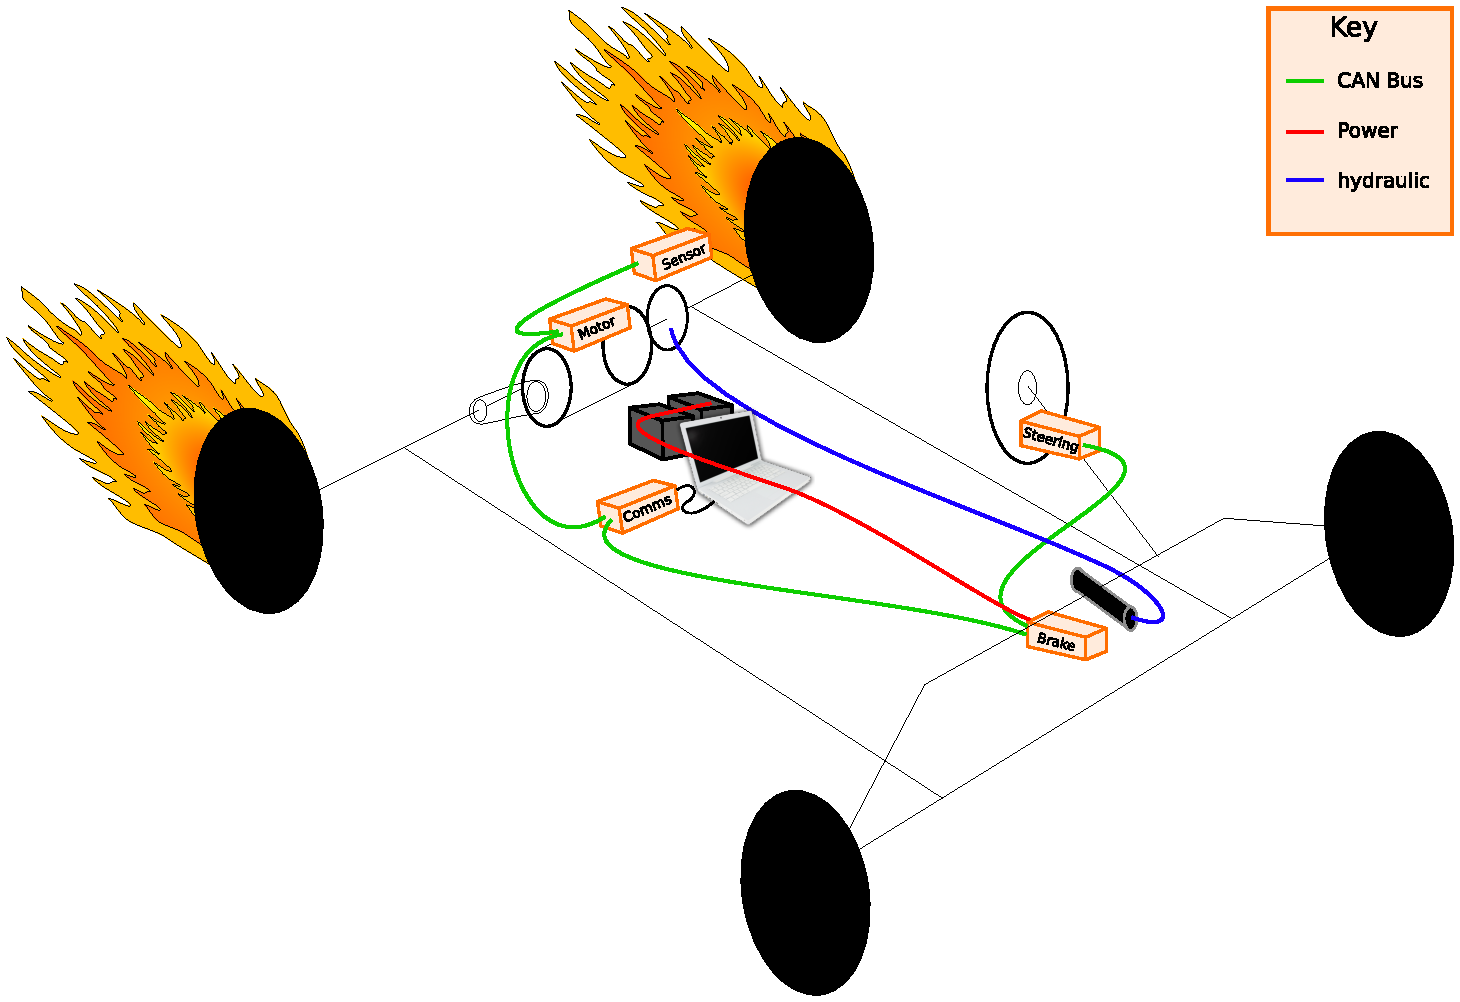
\includegraphics[width=.95\textwidth]{Images/layout}
    \end{center}
\end{frame}

\begin{frame}
\frametitle{How it all communicates}
\framesubtitle{Comms}
CAN Bus
\begin{itemize}
\item Inter-board Communications
\item Expandable if someone wants to add more nodes
\end{itemize}
USART
\begin{itemize}
\item Two on each board
\item One used for debugging
\end{itemize}
SPI
\begin{itemize}
\item Two on each board
\item One 5v level logic
\end{itemize}
USB
\begin{itemize}
\item Fast communication with computer
\end{itemize}
\end{frame}

\begin{frame}
\frametitle{Conclusion}
\framesubtitle{The end\ldots}
\begin{itemize}
\item All Hardware working
  \begin{itemize}
  \item Only 3 minor mistakes on boards
  \item Nice hardware platform for future years
  \end{itemize}
\item Project almost stuck to time plan
  \begin{itemize}
  \item Although we cut the goal down, we came close to achieving our stepping
  stone goal.
  \end{itemize}
\item Project well documented
  \begin{itemize}
  \item Wiki for documentation
  \item Group coding standard adhered to
  \end{itemize}
\item Most of all
  \begin{itemize}
  \item I learnt a lot
  \item Had a heap of fun
  \end{itemize}
\end{itemize}
\end{frame}

%Question frame
\begin{frame}
\begin{center}
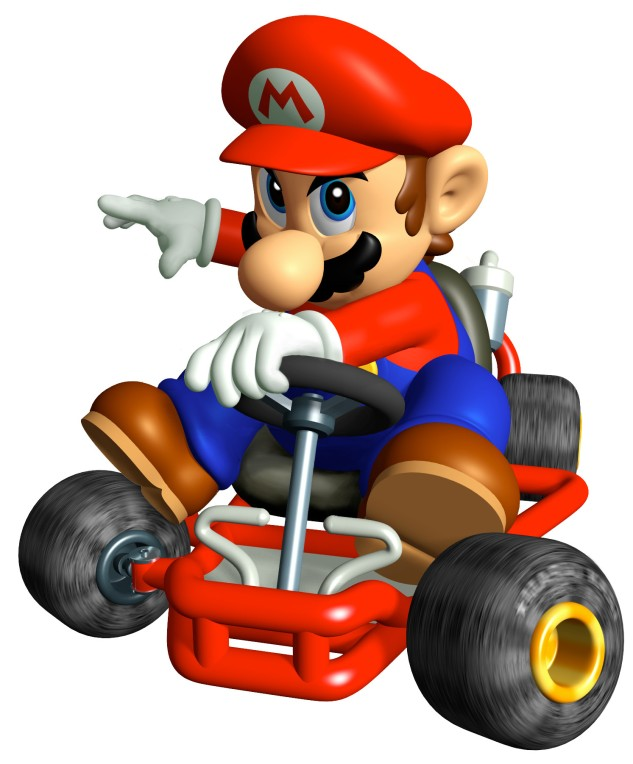
\includegraphics[width=.70\textwidth]{Images/Mario}
\end{center}
\end{frame}


\end{document}
